%% $RCSfile: proj_report_outline.tex,v $
%% $Revision: 1.2 $
%% $Date: 2010/04/23 02:40:16 $
%% $Author: kevin $

\documentclass[11pt
              , a4paper
              , twoside
              , openright
              ]{report}


\usepackage{float} % lets you have non-floating floats
\usepackage{listings}
\usepackage{color}
 
\definecolor{codegreen}{rgb}{0,0.6,0}
\definecolor{codegray}{rgb}{0.5,0.5,0.5}
\definecolor{codepurple}{rgb}{0.58,0,0.82}
\definecolor{backcolour}{rgb}{0.96,0.96,0.95}
 
\lstdefinestyle{mystyle}{
    backgroundcolor=\color{backcolour},   
    commentstyle=\color{codegreen},
    keywordstyle=\color{magenta},
    numberstyle=\tiny\color{codegray},
    stringstyle=\color{codepurple},
    basicstyle=\footnotesize,
    breakatwhitespace=false,         
    breaklines=true,                 
    captionpos=b,                    
    keepspaces=true,                 
    numbers=left,                    
    numbersep=5pt,                  
    showspaces=false,                
    showstringspaces=false,
    showtabs=false,                  
    tabsize=2
}
 
\lstset{style=mystyle}
\usepackage{url} % for typesetting urls

\usepackage{amsmath}
\usepackage{xcolor}
\newcommand\todo[1]{\textcolor{red}{#1}}
%
%  We don't want figures to float so we define
%
\newfloat{fig}{thp}{lof}[chapter]
\floatname{fig}{Figure}

%% These are standard LaTeX definitions for the document
%%                            
\title{Identifying Redundant Test Cases}
\author{Marc Shaw : 300252702}

%% This file can be used for creating a wide range of reports
%%  across various Schools
%%
%% Set up some things, mostly for the front page, for your specific document
%
% Current options are:
% [ecs|msor]              Which school you are in.
%
% [bschonscomp|mcompsci]  Which degree you are doing
%                          You can also specify any other degree by name
%                          (see below)
% [font|image]            Use a font or an image for the VUW logo
%                          The font option will only work on ECS systems
%
\usepackage[image,ecs,behons]{vuwproject}

% You should specifiy your supervisor here with
\supervisors{Dr. David J Pearce and Prof. Lindsay Groves}

% Unless you've used the bschonscomp or mcompsci
%  options above use
%   \otherdegree{OTHER DEGREE OR DIPLOMA NAME}
% here to specify degree

% Comment this out if you want the date printed.
\date{}

\begin{document}

% Make the page numbering roman, until after the contents, etc.
\frontmatter

%%%%%%%%%%%%%%%%%%%%%%%%%%%%%%%%%%%%%%%%%%%%%%%%%%%%%%%

%%%%%%%%%%%%%%%%%%%%%%%%%%%%%%%%%%%%%%%%%%%%%%%%%%%%%%%

\begin{abstract}

\todo{todo}

\end{abstract}

%%%%%%%%%%%%%%%%%%%%%%%%%%%%%%%%%%%%%%%%%%%%%%%%%%%%%%%

\maketitle

\tableofcontents

% we want a list of the figures we defined
\listof{fig}{Figures}

%%%%%%%%%%%%%%%%%%%%%%%%%%%%%%%%%%%%%%%%%%%%%%%%%%%%%%%

\mainmatter

%%%%%%%%%%%%%%%%%%%%%%%%%%%%%%%%%%%%%%%%%%%%%%%%%%%%%%%

% individual chapters included here
\chapter{Introduction}\label{C:intro}

Test suites are becoming an increasing priority within software engineering development areas. Driven by agile methodologies incorporating practices such as test driven development and continuous integration. The use of a test suite is an attempt to cover the majority of situations that may occur. The number of situations is often endless, so covering the majority can incur a large number of tests and in turn take several hours to run. Throughout the project test cases are constantly being added, often when a piece of code is altered, new code is developed or a bug gets fixed. A question arises, how can we ensure that the first test case is not doing the same as the thousandth? Even with careful planning, it is near impossible to have no redundant test cases, which is when a test is nearly or exactly a replication of another test. Therefore, examination of the test cases should occur. 

During a tests execution, a 'paper trail' is left behind. This trail is the method executions that are called during the test, referred to as the tests spectra. A spectra is the set of data that will be analysed using different metrics to determine how related a test is with another. Each tests spectra will be analysed with every other test. Using this analysed information will help identify potential redundant test cases. In figure \ref{fig:spectra} we see the spectra's of three different tests. We clearly can see that Test 1 is different from Test 2 and 3. However, there appears to be similarities between Test 2 and 3 which may need further investigation.

\begin{figure}[h]
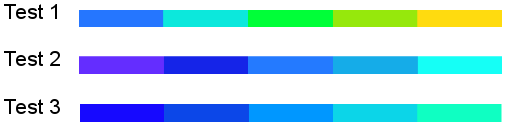
\includegraphics[width=3cm,height=6cm]{spectra.png}
\caption{Spectra}
\label{fig:spectra}
\end{figure}

It is important to understand the dangers of removing test cases. Unless two test cases are exactly the same, it is difficult to guarantee that they are indeed redundant, even if one is a subset of another. Therefore the aim of the project is to identify different approaches that give developers an idea on the number of redundant test cases that are contained within a project. It should allow the developer to run a set of pipelines they specify and view the results on a GUI, allowing manual inspection to determine if they are truly redundant. This means that the tool is useful for gaining an overview and understanding of the condition of the current test suite.

A potential use of the tool is to allow for splitting of any redundant tests into separate test suites allowing for them to be run at different times. For example, one test suite can be run during continuous integration, and the other over night. Ensuring that we are not losing any probability of finding a bug, instead redistributing the test time.

Dr David Pearce is currently writing a language called Whiley, which contains an extended static checking framework in order to eliminate run time exceptions through formal verification techniques. In the compiler module alone, there are roughly 40,000 tests. To reduce this number could result in allowing David Pearce to increase development speed due to a reduction in the time taken to run a large test suite. 
\chapter{Related Work}\label{C:related}

Testing is a critical part to any software engineering process, not only to stop incidents stemming from the the product, but also partially related to the increase in popularity of agile methodologies \cite{chaos}. Many of these methodologies employ test driven development and continuous integration resulting in testing becoming more important throughout the development process. For these reasons there have been research papers that examine the different approaches that can be taken to identify redundant test cases and reduce the size of test suites \cite{wong1995effect, wong1999test, rothermel1998empirical, rothermel2002empirical,koochakzadeh2009test,zhang2011empirical,li2008static}.

It is unclear whether programmatically reducing a test suite's size is worth the tradeoff in the ability to locate bugs.  Wong et al. \cite{wong1995effect, wong1999test} found that test suite reduction does not severely impact fault detection capability. In contrast, Rothermel et al. \cite{rothermel1998empirical, rothermel2002empirical} found that test-suite reduction can severely impact the fault detection capability. This is the reason that our research uses human intuition to have the final say.

A popular technique used in detecting redundancy involves analysing the statement executions, known as coverage information. Maurer, Garousi and Koochakzadeh \cite{koochakzadeh2009test} attempt to answer the question, is coverage based identification enough information to determine redundant test cases? To identify a redundant test case, they state it as being a test case that does not improve a specific criterion. For example, in Figure \ref{fig:venndiagram} we see that according to the coverage data of test cases, T1 ... T5, T4 and T5 are fully redundant as T3 covers the statements that are executed by those tests. This criterion is examining statement coverage. They looked at two other criterion, branch coverage and granularities. Granularity criterion involved splitting the tests into setup, exercise (execution), verify (assert) and lastly teardown then performing analysis over each section. They implemented two different metrics in which both used the criterion described above. These two metrics examined redundancy on at a 1-1 and 1-all relationships. By comparing with manual inspection, they were able to determine the level of false positive and actual redundant tests. Of the redundant tests identified manually, the metrics matched 95\% of those. However, of the tests that were manually identified as being non-redundant, 52\% of these were identified as being redundant by the metrics. They concluded that coverage-based information is vulnerable in giving false-positives when identifying redundant test cases, suggesting common code paths as being the main protagonist. 

\begin{figure}[h]
\begin{center}

\includegraphics[]{VennDiagram.png}
\end{center}
\caption{A Typical Criterion}
\label{fig:venndiagram}
\end{figure}

A technique that Zhang, Marinov, Zhang and Khurshid \cite{zhang2011empirical} examined was the use of a greedy technique in comparison to heuristics with the coverage information. This required a test requirement to be set by the tester, for example using statement coverage. The greedy technique would greedily select a test case that satisfies the maximum number of unsatisfied test requirements and would continue until all the test requirements had been satisfied. So the new test suite will contain exactly the same coverage as the old test suite while removing redundant test cases. This means that if a test subsumed another, then it would always be removed. The heuristic implementation was first conceived by Harrold, Gupta and Soffa \cite{harrold1993methodology} where essential test cases are selected as early as possible. Essential being that only when one test case satisfies a test requirement exclusively. The heuristic approach resulted in the most cost-effective reduction showing that although greedy approach worked, there were better techniques available.

In situations where it is not possible to generate a spectrum to analyse, static analysis can be used to determine the level of redundancy. Robinson, Li and Francis \cite{li2008static} examine the possibility to do this. For the benchmark they use, the test cases are written in a high level automation framework and consist of a list of commands. The commands perform actions such as file copying and loading configurations. To identify redundant test cases they examine the test cases commands as well as the instructions within the procedures that the test case loads. To calculate the similarities between two test cases, they consider three different metrics, Manhattan distance, unigram cosine similarity and bigram cosine similarity. They each were measuring how closely related two tests were based on the sequence of commands and procedures loaded. Their findings were similar to Maurer et al. \cite{koochakzadeh2009test} in that there are a large number of false - positives.

Static checking has several limitations in comparison to dynamic. Firstly, during run-time is when a large part of the paper trail is accessible. Before then the only information available are the method calls. Secondly, it is more difficult to analyse, due to inheritance in many languages adding a complex situation when determining method execution. Static checking therefore would provide useful information in a framework where dynamic data can not be collected and allows for the test cases to be examined in a static fashion such as the one used by Robinson, Li and Francis \cite{li2008static}. Dynamic allows for more data to be collected such as the parameters passed to a method as well as the ability to be executed on more suites. The papers examined looked at the coverage of a test suite at several different criterion levels but none looked at the spectra explicitly. This leaves a potentially useful approach to the problem that may help determine the level of redundancy within a test suite. 
\chapter{Work Done}\label{C:workdone}

\section{Overview}

The ability to trace java unit tests and perform several different analysis metrics has been implemented. For this to be achieved, several factors had to be completed and these are explored in this chapter. The different types of spectra are looked at in Section \ref{S:spectra}. The different types of analysis metrics are explored in Section \ref{S:metrics}. How the tracing is performed is examined in Section \ref{S:trace}, while the creation of the framework is explored in Section \ref{S:framework}. Lastly, how the benchmarks were selected is looked at in Section \ref{S:bench}.

\section{Test Spectra}
\label{S:spectra}

The idea of a spectrum was previously identified in Chapter \ref{C:intro}. A spectrum is some abstraction of the method executions during a test. This allows there to be several different types of spectra. The main three spectra examined are set, list and calling context. An example using the word kitten will be used to show them, where each letter represents a method execution and each letter is from the same parent method.

\begin{itemize}
\item Set of method executions - where every method execution is only taken into account once (Result: 'Kiten')
\item List of method executions - where every method execution is taken into account, including duplicate calls (Result : 'Kitten')
\item Calling Context - for each method call, the data contains a separate node for each call stack that the method was called with \cite{callingcontext} (Result : 'Parent $\rightarrow$ k, Parent $\rightarrow$ i, Parent $\rightarrow$ t ...) 
\end{itemize}
These spectra will be analysed by different metrics to determine the level of redundancy between two tests. This is achieved in Java by examining the stack trace of the method call, where it gives information on the calling tree for that method execution. In the next section, two different analysis metrics are introduced and examined.

\section{Analysis Metrics}
\label{S:metrics}

The first metric is the Levenshtein distance between two tests spectra. This metric is the minimal number of operations that can be done to make one tests spectrum equal to another. These operations are inserting, deleting or substituting method calls and a cost is associated with completing an operation. The max difference is the size of the larger of the two spectra's. The amount of redundancy is calculated by dividing the cost of operations with the max difference in order to normalize the value. This value will be the percentage of tests that are not redundant, we minus this value by 1 to give the redundant level.

If we look at an example using a list spectra, where 'kitchen' is being compared to 'kitten' then we will have to do the following changes.

\todo{Put into a structured table to show more clearly. Unsure how.}
\begin{enumerate}
\item kitten $\rightarrow$ kitcen (Substitution of 't' with 'c')
\item kitcen $\rightarrow$ kitchen (Insertion of 'h' between 'c' and 'e')
\end{enumerate}

This shows the number of operations needed is 2, and the max is 7 as kitchen contains 7 characters. The redundancy is calculated by subtracting 1 from the cost over the max potential cost. So these two words contain 71\% redundant information. 

The second metric was determining the total difference between two spectra. This metric disregarded the calling order of a spectra, which is comparable to looking at the coverage as done in several papers \cite{fraser2007redundancy,koochakzadeh2009test,zhang2011empirical,jeffrey2005test}. The metric sorts the method calls of a spectra in alphabetical order and increments a value by 1 for each difference there is between two tests spectra. Resulting in the total difference between two tests. This value is then divided by the max possible value, which would occur when every method call is different becoming the length of both spectra, to produce a normalized redundancy value. This metric is also minimization.

Using the same spectra example as above, we need to rearrange 'kitchen' and 'kitten' into alphabetical order before calculating the redundancy, 'cehiknt' and 'eikntt' respectively.

\todo{Put into a structured table to show more clearly. Unsure how.}
\begin{enumerate}
\item Remove 'c' from 'cehiknt', increment value by 1
\item 'e' is contained in both, remove from both
\item Remove 'h' from 'hiknt', increment value by 1
\item 'iknt' is contained in both, remove from both
\item Remove 't' from 't', increment value by 1
\end{enumerate}

The total difference between the two is 3. While the max would be if they were both completely different which is 13. The redundancy is calculated by subtracting 1 from the cost over the max potential cost. The outcome being that the two words are 77\% redundant.

Maurer et al. \cite{koochakzadeh2009test} and Robinson et al. \cite{li2008static} found that test cases often had a set of methods that were in every test, such as setup and tear down. These common methods could create false positives. To understand why, a redundant test is one where it is nearly or exactly a replication of another test. Since each method call within an spectra has the same weighting, the more setup and teardown calls made means that the execution stage has decreased weighting overall. So the idea in weighting is to increase the 'importance' of lower frequency method calls by discarding the top 20\% method calls. This weighting will be added into a spectrum, where the spectrum will ignore the top 20\% method calls.

\section{Tracing}
\label{S:trace}

David Pearce's language Whiley is written in Java. Therefore it was decided to use Java to trace a tests spectrum. There are two viable options, the Java Debugging Interface (JDI) or AspectJ. JDI is similar to using an observer pattern. When a method is called, the listening trace class will be notified. In contrast, AspectJ utilises byte code weaving; this is when a piece of code is added to existing code without modifying the code itself. It uses a point cut to identify what code is weaved and where in the code \cite{aspectwiki}. A point cut is made in every method call, this point cut calls a static method in a tracer class, passing it the information about the method execution. AspectJ allows for several methods to achieve tracing through byte code weaving:

\begin{itemize}
\item Compile time:
The classes are compiled with the aspect weaved into them. So that when the jar is executed, the methods have the byte code from the aspect weaved into it already.
\item Load time:
This involves binary weaving deferred until the point in which a class loader will attempt to load in a class file.
\end{itemize}

Load time allowed for ease of use when working with external benchmarks as it only required AspectJ's class loader to be used instead through a command line flag of rebuilding the benchmarks with the AspectJ compiler.

In regard to JDI or AspectJ, AspectJ allows for more ability to choose which methods to record and making it easier to retrieve parameter values, JDI was faster to execute but provided less documentation. The decision to use AspectJ was based off this trade off between more information and performance. The analysis framework was able to be altered to increase the performance of it, so having the extra information that AspectJ gave was more important than an taking less time to execute.

\section{Framework}
\label{S:framework}

The spectrum of every test has to be compared to that of every other test in order to identify redundant test cases. The metrics identified become computationally heavy with thousands of test cases containing a spectrum consisting of tens of thousands of methods calls. To perform an analysis on that scale would take several days. A pipeline combined with time reduction strategies was determined to be the best solution.

A pipeline approach is shown in Figure \ref{fig:pipeline}. The analysing stages can be set by the user within a properties file, where they can select the spectra type, analysis metric to use and level of redundancy for each. This allows execution of reduction strategies before executing more computationally heavy analysis.

\begin{figure}[h]
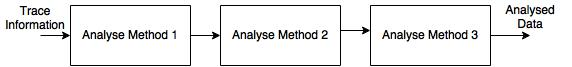
\includegraphics[width=\textwidth]{Pipeline.jpg}
\caption{Trace information goes in at the start of the pipeline. After each stage there will be a reduction of comparisons that the next stage has to complete. The last stages should be the most computationally heavy.}
\label{fig:pipeline}
\end{figure}

There were two approaches that were used to reduce the amount of analysis time. They were - implementing a heuristic and using concurrent execution. 

The heuristic looked at set of method calls, rather than a list. This meant the number of comparisons decreased. Using a 99 percent similarity for the heuristic on the wyc package of Whiley, this decreased the comparisons from stage 1 having 187922 to stage 2 with 232. 

The following illustrates an example of this.

$K,I,T,C,H,E,N \neq K,I,T,E,N,Z $

In this case, the two test cases would not be redundant due to them having a large difference in method calls.

$K,I,T,C,H,E,N \approx K,I,T,C,H,N$

There is a chance that these two may be redundant so it implies more computational heavy analysis should be done, such as analysing the list spectra. 

Concurrent execution was implemented by splitting the test cases up into 8 different parts, each part knew the test cases that it had to compare. A new thread was run to execute the comparisons, making the implementation relatively easy. The concurrent execution lead to a decrease in roughly 2 times the time taken to analyse the spectra's but lead to a trade off in an increased memory usage. This meant concurrent execution was only usable for the smaller bench marks.
Another issue was that for each analysis of a benchmark, the tests had to be rerun, this could take several hours. The solution was to save the spectra data to disk. This ensured that a distributed computing system (ecs grid) could be used to execute data analysis, meaning that 150 analysis jobs could be run at once.

Using reflection will allow for retrieval of parameter values, the use of parameters allows for more certainty about the whether two tests are redundant. The most common use case would involve the use of parameters therefore it was decided to optimize this through storing the data with parameters. The optimization involved saving the parameters with the trace information. If parameters value is set to false, the parameters have to be split off rather than added on. This means that setting the parameters to false would increase the set up time.

\section{Benchmarks}
\label{S:bench}
Suitable benchmarks had to be found to test the different metrics on. They were located by looking at popular java framework's, Github repositories and David Pearce's personal projects. The benchmarks had to meet a criteria where they were Java based, had reasonable number of tests (40+) and were open source. Although there were over ten potential benchmarks, the ability to use them depended on their build process. If they used Maven, it was difficult to create a jar that contained the tests and often meant that the amount of effort needed to get a working benchmark was higher than the benefit from it. This eliminated several potential benchmarks and left the Ant and gradle built projects. In Table \ref{large_test} we see the large bench marks used. These involved bench marks that required more than \todo{TODO} number of comparisons. The type of tests were also taken into consideration.

The current set of benchmarks is as follows:
\begin{table}[]
\centering
\caption{Large Test Suites}
\label{large_test}
\begin{tabular}{|l|l|l|l|}
\hline
{\bf Benchmark}       &  {\bf Number of Tests} & {\bf Type of tests} & {\bf Authors}   \\ \hline
Whiley - Wyc Valid         &       &    End to End      & David J Pearce          \\ \hline
Spring - Core   &       &    Unit Tests      & Community \\ \hline
Metric-x - Core &       &    Unit Tests      & Community \\ \hline
Ant             &       &    Unit Tests      & Community \\ \hline
\end{tabular}
\end{table}

\begin{table}[]
\centering
\caption{Small Test Suites}
\label{small_test}
\begin{tabular}{|l|l|l|l|}
\hline
{\bf Benchmark}   & {\bf Number of Tests} & {\bf Type of tests} & {\bf Authors}  \\ \hline
Jasm              &             &    End to End      & David J Pearce \\ \hline
Imcache &           &    End to End        & Community \\ \hline
\end{tabular}
\end{table}

\chapter{Future Work and Conclusions}\label{C:future}

This chapter will first discuss potential future work which would increase the usefulness of the tool for a wider range of audiences. The experiments are then reflected on and finally concluded. 

\section{Future Work}
Throughout the project, three main areas have been identified for future work: The ability to handle larger test suites, tracing statement information and lastly, using both statement and method information together.

\begin{itemize}

\item \textbf{Handle larger test suites.} The main objective would be to increase the ability of the tool to handle larger test suites. Currently, the tool relies on RAM to hold the trace and analysis information however, the amount of data held can often grow rapidly if the test cases contain a large number of method calls. An approach to get around this would be to integrate the tool with a database. \todonote{This was achieved in Nelsons.....} This would allow the tool to handle arbitrary large suites. The down side would that the speed of the tool would decrease as the read/write to disk is slower than to RAM. This may be negligible as databases optimize their read and write by using a certain amount of memory. Giving developers this option would increases the capability of the tool. 

\item \textbf{Trace statement information.} The tool has the ability to trace method call information and has potential to be used on large test suites. This approach may not be the best when we are only looking at smaller test suites. Another approach that could be implemented is tracing the statement coverage information. This would allow us to compare the statement and method coverage information directly and give us more insight into the issue of identifying redundant tests. Tracing the statement information would allow us to further explore the use case mentioned in Chapter \ref{C:intro}. The use case was the ability to split the test suites into two, one containing the non redundant test cases and the other was the original suite. This could be further expanded with statement coverage information. By identifying when a test subsumes another, the test subsumed could be moved into another suite. If the larger test fails, the subsumed tests could then be ran to help pin point the error in the code.

\item \textbf{Combining Statement and method information.} The method call information was a good heuristic to use. On the other hand, it is difficult to judge how good method calls are at identifying redundant test cases without any comparison to statement coverage or large scale redundancy and bugs added. One application could be to combine the statement and method information together. The tool could use the method information as a heuristic and statement coverage could then explore the test cases identified by the heuristic.

\end{itemize}

\section{Conclusions}

There were two main contributions of the paper as discussed in Chapter \ref{C:intro}:

\begin{itemize}
\item Create a tool for identifying redundant test cases (Chapter 3)
\item Analyse different strategies for identifying redundant test cases through experimenting on realistic benchmarks (Chapter 4)
\end{itemize}

Throughout the report, the tool has been discussed along with the different techniques implemented. The tool first had to trace the data. This was achieved through the AspectJ framework. After the test suites were able to be traced, the trace information then had to be filtered with different spectra. The ability to filter out information was one of the key features of the tool. This allowed developers to trace information, then run a range of different filters over the data without being constrained to one spectra. The three spectra filters were ``unique method calls", ``all method calls" and "call tree". The other key feature of the tool was the pipeline. Integrating it with the spectra filters allowed for the "unique method calls" to be used as a heuristic to reduce the number of comparisons that the subsequent stages had to perform. The tool then was altered to trace the parameter information from the test cases. This was achieved by using reflection on the parameter objects. Finally, the ability to apply a weighting was implemented. This was achieved by removing the top 20\% method calls.

\paragraph{Method Call Information}
The use of method call information was a good candidate to identify redundant tests. They allow the tool to look at test suites that produce a larger amount of total information, in particular ones which are end to end tests -- Whiley and Jasm. As mentioned in the Future Work section above and discussed in Experiment \rom{2}, the method calls appeared to be particularly good at being used as a heuristic. Filtering with the "unique method calls" spectra, the tool was able to remove a large portion of the test case comparisons in the final stage had to perform while retaining good precision.

\paragraph{Pipeline}
Pipelining was one of the critical aspects of the project. It not only lead to a decrease in the time taken but also the memory consumed. An important thing to note is each benchmark had an optimal length of the pipeline, using a length larger than the optimal caused more time to be taken to analyse than was saved. Pipelining particularly worked well with the use of a "unique method call" spectra filter.

\paragraph{Call tree depth}
The experiments showed that as the depth of the call tree increased, there was limited level of reduction in the number of redundant tests identified. This result was unexpected. Although there was a change, it was lower that what was expected. This implies that by increasing the K depth without any other technique, there is limited improvement. 

\paragraph{Parameter}
By using reflection to retrieve the fields of these objects it allowed more insight into the content that the parameter objects were holding and the nature of them, but it also meant more data had to be held and analysed resulting in an increased time taken. There exists this trade off between time taken and confidence of redundancy when using parameters. 

\paragraph{Weighting}
The weighting technique implemented attempts to improve the accuracy of the tool by removing false-positives while improving the time taken to analyse. Experiment \rom{4} discussed how weighting was able to reduce the level of false-positives but needs further improvement.

\paragraph{}
The project has explored the use of higher level information than previously explored for identifying redundant test cases while examining how different techniques can impact the results. The output of the tool is adequate in the sense that there is a low number of tests identified and these tests contain limited non-redundant tests. 




%%%%%%%%%%%%%%%%%%%%%%%%%%%%%%%%%%%%%%%%%%%%%%%%%%%%%%%

\backmatter

%%%%%%%%%%%%%%%%%%%%%%%%%%%%%%%%%%%%%%%%%%%%%%%%%%%%%%%


%\bibliographystyle{ieeetr}
\bibliographystyle{acm}
\bibliography{sample.bib}


\end{document}
